%%%%%%%%%%%%%%%%%%%%%%%%%%%%%%%%%%%%%%%%%%%%%%%%%%%%%%%%%%%%%%%%%%%%%%%%
\chapter{Techniques for Fetal Brain Segmentation} \label{chap:TechniquesForFetalBrainSegmentation}
%%%%%%%%%%%%%%%%%%%%%%%%%%%%%%%%%%%%%%%%%%%%%%%%%%%%%%%%%%%%%%%%%%%%%%%%
\vspace{1cm}

Automated segmentation of the fetal brain is a central task in the analysis of prenatal MRI, furnishing an anatomical framework for studying brain development and enabling quantitative measurements. Manual annotation, while considered the reference standard, is time-consuming, requires expert knowledge, and suffers from inter-observer variability. Consequently, a wide range of computational approaches have been developed to achieve accurate, reproducible, and efficient segmentation of fetal brain structures.

Over the years, segmentation methods have evolved from traditional atlas-based strategies to modern deep learning approaches. Atlas-based techniques leverage anatomical priors by registering subject images to predefined templates, but often struggle with variability in fetal brain size, orientation, and image quality. More recently, convolutional neural networks have emerged as the dominant paradigm, outperforming classical approaches while remaining sensitive to differences in acquisition protocols, scanners, and populations. Domain generalization addresses the challenge of adapting models to these variations, ensuring robust performance across diverse imaging conditions.

This chapter reviews the main methods for fetal brain segmentation, introducing the concept of domain generalization and presenting the state of the art. Ultimately, it outlines the most recent results of the FeTA Challenge, which provides a benchmark for evaluating segmentation methods in a standardized setting.

\section{Domain Generalization} \label{sec:DomainGeneralization}
In medical image segmentation, a \emph{domain} encapsulates both the feature space and the underlying marginal distribution of imaging data. Domain shifts arise when models trained on one domain are tested on data from another dataset. In medical imaging, the most prevalent sources of domain shift arise from variations in image acquisition processes, encompassing differences in imaging modalities, scanning protocols, and device manufacturers---a more exhaustive description of the potential sources can be found in Section \ref{sec:Challenges}. This is frequently referred to as \enquote{acquisition shift}. Unlike data generalization, where test samples share the same distribution as training data, domain generalization addresses the scenario where test data arise from a distinct, unseen domain\,\cite{Ouyang2023}.

Domain generalization (DG) methods can be categorized into three main groups, which are often complementary and can be combined to achieve higher performance\,\cite{Wang2023}:
\begin{description}
    \item[Data Manipulation] These methods focus on manipulating input data to assist in learning general representations. The primary objective is to increase the diversity and quantity of existing training data.
    \begin{itemize}
        \item \textbf{Data Augmentation-Based DG:} This involves applying various transformations to training data  to simulate different domain characteristics and reduce overfitting. Domain randomization is a common technique where new data is generated by introducing random variations in parameters such as object location, texture, shape, number, illumination, camera view, and noise. An example in medical imaging is SynthSeg\,\cite{Billot2023}, which generates synthetic images with randomized contrasts based on Gaussian mixture models (GMMs), along with geometric deformations and resampling to simulate different image resolutions. FetalSynthSeg\,\cite{Billot2023} further extends this by incorporating intensity clustering and meta-classes for fetal brain MRI. Another approach is adversarial data augmentation, which generates image perturbations that are specifically designed to easily flip the predictions of classifiers, thereby making the model more robust to such changes.
        \item \textbf{Data Generation-Based DG:} It involves creating diverse and rich synthetic data to boost a model's generalization capabilities. Techniques often leverage generative models such as variational auto-encoders (VAEs) and generative adversarial networks (GANs), or strategies like Mixup\,\cite{Zhang2018}. These methods can be complex due to their computational demands and the careful design required for the generative models.
    \end{itemize}
    \item[Representation Learning] This category aims to learn feature representations that are robust to domain shifts. The core idea is to decompose the prediction function into a feature extraction (representation learning) function and a classifier function, focusing on making the feature extraction robust.
    \begin{itemize}
        \item \textbf{Domain-Invariant Representation Learning:} This approach seeks to reduce the discrepancies between feature distributions across multiple source domains. The underlying principle is that if feature representations remain invariant to different domains, they are inherently more general and transferable to unseen domains. This involves methods like kernel-based methods\,\cite{Blanchard2021}, domain adversarial learning---e.g., domain-adversarial neural networks, DANN \cite{Ganin2015, Ganin2016}--- and invariant risk minimization (IRM)\,\cite{Krueger2021}.
        \item \textbf{Feature Disentanglement-Based DG:} It aims to separate learned features into domain-shared features---which are common across domains and useful for the task---and domain-specific features---which capture domain-specific variations. In this category, causality-inspired methods aim to ensure that the learned representations capture the \enquote{true cause} of the labels (e.g., object shape) and are therefore unaffected by correlated but irrelevant features like background, color, or style. Causality-inspired methods have been used to achieve single-source domain generalization through data augmentation. The idea is to simulate interventions on irrelevant features, thereby exposing the network to synthetic acquisition-shifted training examples.
    \end{itemize}
    \item[Single-Source Domain Generalization (\textsc{ssdg})] This is a specific and highly challenging setting within domain generalization where only a single source domain is available for training. This scenario is particularly common in medical imaging applications due to the high cost of data collection, privacy concerns, and scarcity of diverse datasets\,\cite{Ouyang2023}. The key to this problem is to generate novel domains using data generation techniques to increase the diversity and informativeness of training data\,\cite{Wang2023}. The performance degradation that deep learning models face due to domain shift can be attributed to\,\cite{Ouyang2023}:
    \begin{itemize}
        \item \textbf{Shifted Domain-Dependent Features:} Image appearances, including intensities and textures, are inherently domain-dependent. Deep networks are acutely susceptible to shifts in these features. In contrast, human annotators can readily identify anatomical structures across different domains by focusing on domain-invariant shape information, which is intuitively causal to segmentation masks, unlike intensity or texture.
        \item \textbf{Shifted-Correlation Effect:} Due to confounding variables, objects in the background of an image may be spuriously correlated with the objects of interest, rather than causally related. For example, a network might learn that a certain background artifact (which, in the case of fetal MRI, would be the skull and the maternal tissues) is correlated with a specific anatomical structure within a source domain. If this artifact is absent or appears differently in an unseen target domain, the network's reliance on this spurious correlation can lead to failure.
    \end{itemize}
The goal of \textsc{ssdg} is to mitigate these effects by steering the network towards learning domain-invariant features, such as shape information, and immunizing the segmentation model against the shifted-correlation effect by removing confounders during training. This is exactly the idea behind \textsc{gin-ipa}\,\cite{Ouyang2023}, that is discussed in greater detail in Section \ref{sec:Challenges}.
\end{description}

\section{Atlas-based Methods}

\section{Convolutional Neural Networks}
% U-Net
% State of the art

\section{The FeTA Challenge}
The Fetal Tissue Annotation Challenge (FeTA)\,\cite{FeTA2024} was born in 2020, and joined the International Conference on Medical Image Computing and Computer-Assisted Intervention (\textsc{miccai})\,\cite{MICCAI} in 2021. Up to now, four editions have been organized (in 2020, 2021, 2022, and 2024), with increasing participation and interest from the medical imaging community. The main contributions of the FeTA challenge are the creation of a benchmark dataset for fetal brain MRI segmentation and biometry, and the promotion of the development of algorithms for the automatic segmentation of fetal brain tissues.

The main task in FeTA is the segmentation of brain tissues in fetal MRI, which is a challenging problem due to the low contrast between tissues, the presence of noise, and the variability in the shape and size of the fetal brain. The dataset used in the challenge is composed of 3D super-resolution (SR) reconstructions of 2D fetal brain MRI images. Participants are asked to segment the fetal brain into seven tissues: external cerebrospinal fluid (CSF), cortical gray matter (cGM), white matter (WM), ventricles (including cavum), cerebellum, deep gray matter (dGM), and brainstem (BS). The performance is evaluated using three metrics: the Dice similarity coefficient (DSC), the volume similarity (VS), and the Hausdorff 95 distance (HD95). The use of three metrics helps to reduce the reliance on any one metric, which may be misleading in the evaluation of the algorithms\,\cite{FeTA2024_paper}.

The first edition of the FeTA challenge was organized in 2020, by Payette et al.\,\cite{Payette2021}. The challenge consisted in segmenting fetal brain MRI T2w images. The initial FeTA dataset comprised \num{40} super-resolution (SR) reconstructions with manual segmentations for training and \num{10} SR reconstructions without manual segmentation for validation, encompassing both pathological and non-pathological cases. The gestational age (GA) range spanned from \numrange{20}{33} weeks. This dataset established a standard in fetal brain tissue parcellation---according to the seven-tissues protocol previously introduced in\,\cite{Payette2020}---that would be used in all the following FeTA editions. Four research groups participated, submitting a total of ten algorithms. All the algorithms had more or less the same issues in segmenting the CSF---especially for the pathological cases, because of not clear tissue boundaries---and the GM, because of its rapidly changing structure.
The dataset used in the first FeTA edition had important limitations:
\begin{itemize}
    \item Manual segmentations were based on a single segmentation due to time and resource limitations, without consensus delineation.
    \item The data were from one single center, the University Children's Hospital Zurich (Kispi), thus limiting the generalizability of the results.
    \item The images had varying quality grades, with younger GAs and pathological cases often having lower quality.
\end{itemize}

The 2021 edition of the FeTA challenge\,\cite{FeTA2021_review, FeTA2021} was the first to join the \textsc{miccai} conference. The dataset---hereinafter referred to as Kispi dataset---was expanded to \num{120} scans from the same institution, with GAs ranging from \numrange{20}{35} weeks. The acquisition was carried out at \qty{1.5}{\tesla} for a subset of cases, and at \qty{3}{\tesla} for another subset of cases. \num{60} scans were reconstructed with the \textsc{mialsrtk} method\,\cite{Tourbier2015, MIALSRTK}, while the other \num{60} cases with the \textsc{simple irtk} method\,\cite{Kuklisova2012, irtk-simple}. For each reconstruction method, \num{40} cases were included in the training dataset available to the challenge participants (for a total of \num{80} cases), and \num{20} cases were included in testing dataset not available to the participants (for a total of \num{40} cases). \num{21} algorithms were submitted, of which \num{19} were U-Nets, with no major differences in the architecture. Overall, the most challenging labels to segment were cortical and deep GM---due to limited image resolution and annotation uncertainty---and brainstem---especially in the pathological cases. The results of the image quality and SR reconstruction methods are related to each other, as the majority of the low quality images were done with the \textsc{mialsrtk} method, and the excellent quality brain volumes included were reconstructed with the \textsc{simple irtk} method.

FeTA 2022\,\cite{FeTA2022_review, FeTA2022} introduced a multi-center dataset to address the generalizability of algorithms, which was one of the main limitations of the previous editions. In addition to Kispi, data from Medical University of Vienna was incorporated into both the training and testing datasets. Data from two further centers were included in the testing dataset---University Hospital Lausanne (\textsc{chuv}), and Benioff Children's Hospital (UC San Francisco, \textsc{ucsf})---for a total of four centers.
\comment{
(Tab\,\ref{tab:FeTA2022_dataset}).

\begin{table}[htbp]
    \centering
    \begin{tabular}{c|c|c|c|c}
        \toprule
        \textbf{Inst.} & \begin{tabular}{@{}c@{}} \textbf{Scanner} \\ \textbf{(field strength in Tesla)} \end{tabular} & \textbf{SRR method} & \begin{tabular}{@{}c@{}} \textbf{TR/TE} \\ \textbf{(ms)} \end{tabular} & \begin{tabular}{@{}c@{}} \textbf{GA range} \\ \textbf{(weeks)} \end{tabular} \\ \midrule
        \multicolumn{5}{c}{\textbf{Training}} \\
        \midrule
        Kispi & \begin{tabular}{@{}c@{}} GE Signa Discovery \\ MR450/MR750 (1.5/3)* \end{tabular} & \begin{tabular}{@{}c@{}} \textsc{mialsrtk} (40) \\ \textsc{simple irtk} (40) \end{tabular} & \begin{tabular}{@{}c@{}} 2000-3500 \\ 120** \end{tabular} & 20.0-34.8 \\ \hline
        Vienna & \begin{tabular}{@{}c@{}} Philips Ingenia/Intera (1.5) \\ Philips Achieva (3) \end{tabular} & \textsc{NiftyMIC} (40) & \begin{tabular}{@{}c@{}} 6000-22000 \\ 80-140 \end{tabular} & 19.3-34.4 \\
        \midrule
        \multicolumn{5}{c}{\textbf{Testing}} \\
        \midrule
        Kispi & \begin{tabular}{@{}c@{}} GE Signa Discovery \\ MR450/MR750 (1.5/3)* \end{tabular} & \begin{tabular}{@{}c@{}} \textsc{mialsrtk} (20) \\ \textsc{simple irtk} (20) \end{tabular} & \begin{tabular}{@{}c@{}} 2000-3500 \\ 120** \end{tabular} & 21.3-34.6 \\ \hline 
        Vienna & \begin{tabular}{@{}c@{}} Philips Ingenia/Intera (1.5) \\ Philips Achieva (3) \end{tabular} & \textsc{NiftyMIC} (40) & \begin{tabular}{@{}c@{}} 6000-22000 \\ 80-140 \end{tabular} & 18.1-35.0 \\ \hline
        \textsc{chuv} & \begin{tabular}{@{}c@{}} Siemens \textsc{magnetom} \\ Aera (1.5) \end{tabular} & \textsc{mialsrtk} (40) & \begin{tabular}{@{}c@{}} 1200 \\ 90 \end{tabular} & 21.0-35.0 \\ \hline
        \textsc{ucsf} & \begin{tabular}{@{}c@{}} GE Discovery \\ MR750/MR750W (3) \end{tabular} & \textsc{NiftyMIC} (40) & \begin{tabular}{@{}c@{}} 2000-3500 \\ 100** \end{tabular} & 20.0-35.1 \\
        \bottomrule
    \end{tabular}
    \caption{Training and testing dataset properties in FeTA 2022. In parenthesis, next to each SRR method, is reported the correspondent number of images. *The field strengths respectively refers to the scanners. **TE values represent the minimum durations.}
    \label{tab:FeTA2022_dataset}
    \end{table}
}

\num{17} algorithms were submitted, among which nnU-Net was the most used and effective tool. Overall, the median performance metrics in the OOD setting remained equivalent to the in-domain, but for some labels---ventricles, GM and  WM---an important drop in performance was observed. The most challenging labels to segment remained cortical and deep GM, and BS. Notably, some algorithms performed better in the OOD setting than in the in-domain setting. This can be explained with the better quality of the images from the \textsc{chuv} and \textsc{ucsf} centers, which were included only in the test set. Style and photometric augmentations (contrast, blur, sharpness, etc.) turned out to be effective in improving the generalization of the models. However, \enquote{the optimum choice of augmentation techniques remains unclear}\,\cite{FeTA2022_review}, standing as a critical factor in achieving domain generalization. The paper traces a path for future research, highlighting that it should focus on enhancing the generalizability of the methods and that \enquote{conducting a more comprehensive evaluation of the impact of data augmentation and possible biases due to super-resolution reconstruction methods would be very valuable}\,\cite{FeTA2022_review}.

Finally, in FeTA 2024\,\cite{FeTA2024_review, FeTA2024} \num{20} new scans were added to the test set, in order to have more results on the OOD performance. These scans were acquired at St.\ Thomas Hospital (King's College London, KCL), with field strength of \qty{0.55}{\tesla} (Siemens \textsc{magnetom} Free.Max)\,\cite{FeTA2024_paper}. This decision follows the recent rise in popularity of low-cost low-field MRI systems\,\cite{Aviles2023}, which are particularly suitable for fetal imaging due to their lower SAR and acoustic noise\,\cite{Ponrartana2023}. \num{16} algorithms were submitted, of which nine were based on nnU-Net\,\cite{nnUNet, Isensee2021}. The top team used an nnU-Net with a denoising autoencoder, generating ensemble predictions from different models. The second top team used a custom U-Net variant, training it on real and synthetic data (SynthSeg\,\cite{Billot2023}), and applying post-processing to discard non-brain tissues from the predictions. All top-three teams applied extensive data augmentation, combinations of standard augmentations, and model ensembling.

Across the leading methods, average DSC plateaued between \numlist{0.80;0.82}, likely due to the quality of both SRR algorithms and manual segmentations\,\cite{FeTA2022_review}. No statistically significant improvement was observed in overall segmentation performance metrics over the last three editions, suggesting that a performance plateau has been reached despite the increasing sophistication of methodologies and dataset diversity. These results indicate that merely architectural modifications are unlikely to produce significant improvements, consistent with observations from other challenges in which U-Net-based methods frequently outperform more complex designs\,\cite{Eisenmann2023, FeTA2024_review}. Notably, the low-field MRI dataset from KCL achieved the highest segmentation performance among all sites. Conversely, the Kispi dataset, in spite of being an in-domain dataset, exhibited the lowest performance. Although domain shifts are widely recognized as a key challenge for deep learning methods in medical imaging\,\cite{Dockes2021}, the sources of these shifts are rarely disentangled. Analysis of domain shifts revealed that image quality was the most influential factor affecting model generalization, leading to Dice score differences of up to \num{0.10} between low- and high-quality scans. The choice of the SRR pipeline also exerted a substantial impact on segmentation performance, highlighting the need for better modeling of artifacts specific to fetal brain SR pipelines\,\cite{Sanchez2024}. Other factors, such as gestational age, pathology, and acquisition site, contributed marginally to performance variability.

\comment{
\begin{figure}[htbp]
    \centering
    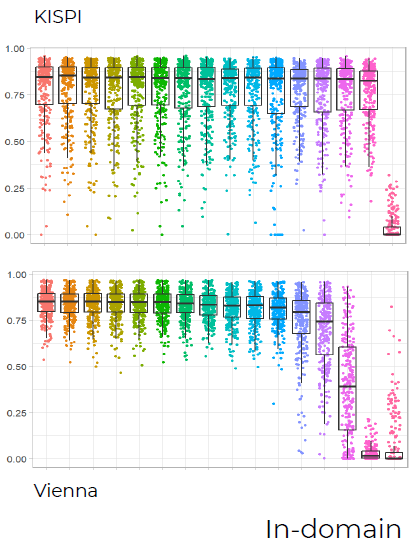
\includegraphics[width=0.4\textwidth]{figures/feta24_in-domain.png}
    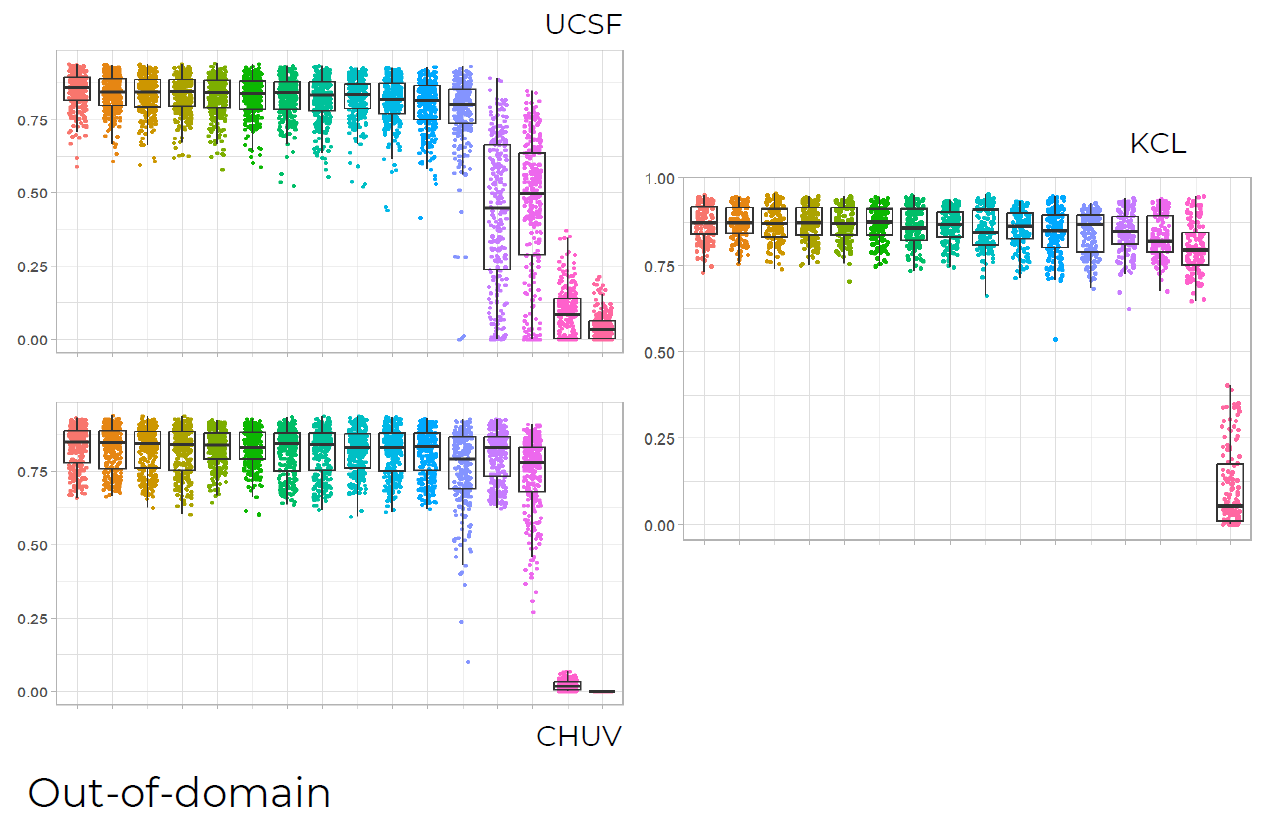
\includegraphics[width=0.8\textwidth]{figures/feta24_out-of-domain.png}
    \caption{Teams' Dice similarity scores in FeTA 2024. From\,\cite{FeTA2024}.}
    \label{fig:FeTA2024_results}
\end{figure}
}